\njustchapter[光催化膜分离反应装置工艺特性研究]{阳极氧化锡的生长模型和多孔氧化锡的电容性能}
\label{chap:experiment-sample}

\section{研究现状分析}

当今，纳米二氧化锡材料在染料敏化太阳能电池、气体传感器、锂离子电池、光电催化等领域具有潜在的应用价值。为了提高材料的稳定性和响应速度，研究者通常从晶体结构、缺陷调控、界面反应和测试装置四个方面展开分析。文献\cite{devillez2007tool,bhatia2024unit} 展示了实验信号检测和自动化分析方法在工程研究中的应用价值，可为本课题的数据处理流程提供参考。

\section{实验过程}

\subsection{纳米多孔氧化锡层的合成}

锡箔（纯度 99.99\%，厚度 100μm）作为阳极氧化的起始材料。实验前依次使用无水乙醇、去离子水清洗样品表面，并在氮气气氛下吹干。阳极氧化过程中保持电解液温度恒定，通过调整电压和反应时间获得不同孔径与厚度的氧化层。

\begin{table}[htbp]
  \centering
  \caption{MGratio 在不同沉积时间下电化学参数的模拟得到的 EIS 结果}
  \label{tab:eis}
  \begin{tabular}{ccc}
    \toprule
    样本 & $R_{\mathrm{L}}$ ($\Omega\ \mathrm{cm}^{-2}$) & $C_{\mathrm{s}}$ ($\mathrm{F}\ \mathrm{g}^{-1}$) \\
    \midrule
    MG4(500s) & 0.564 & 128.4 \\
    MG4(1000s) & 0.539 & 136.7 \\
    MG4(1500s) & 0.564 & 132.1 \\
    \bottomrule
  \end{tabular}
\end{table}

\begin{table}[htbp]
  \centering
  \caption{不同阳极氧化条件下多孔氧化锡结构参数的四线表示例}
  \label{tab:four-line}
  \begin{tabular}{ccccc}
    \toprule
    \multirow{2}{*}{电压/V} & \multirow{2}{*}{时间/s} & \multicolumn{2}{c}{形貌参数} & \multirow{2}{*}{$C_{\mathrm{s}}$/(F g$^{-1}$)} \\
    \cmidrule(lr){3-4}
     &  & 孔径/nm & 厚度/\textmu m &  \\
    \midrule
    3 & 600 & 42.1 & 1.8 & 118.6 \\
    4 & 600 & 55.8 & 2.3 & 136.7 \\
    5 & 600 & 67.3 & 2.9 & 129.4 \\
    \bottomrule
  \end{tabular}
\end{table}

\section{实验方法}

锡箔（纯度 99.99\%，厚度 100μm）作为阳极氧化的起始材料。实验前依次使用无水乙醇、去离子水清洗样品表面，并在氮气气氛下吹干。阳极氧化过程中保持电解液温度恒定，通过调整电压和反应时间获得不同孔径与厚度的氧化层。

\begin{algorithm}[htbp]
  \caption{阳极氧化参数筛选流程}
  \label{alg:anodizing-search}
  \begin{algorithmic}[1]
    \Require 电压集合 $V$，氧化时间集合 $T$，目标孔径 $d_0$
    \Ensure 推荐实验参数 $(v^*, t^*)$
    \State 初始化最小偏差 $\Delta_{\min} \leftarrow +\infty$
    \ForAll{$v \in V$}
      \ForAll{$t \in T$}
        \State 制备样品并测量平均孔径 $d(v,t)$
        \If{$|d(v,t)-d_0| < \Delta_{\min}$}
          \State 更新 $\Delta_{\min} \leftarrow |d(v,t)-d_0|$
          \State 记录 $(v^*, t^*) \leftarrow (v,t)$
        \EndIf
      \EndFor
    \EndFor
    \State \Return $(v^*, t^*)$
  \end{algorithmic}
\end{algorithm}
\FloatBarrier

算法~\ref{alg:anodizing-search} 可以进一步写成简单的数据筛选程序，示例见\njustcoderef{code:parameter-search}。

\begin{lstlisting}[style=mypython,caption=阳极氧化参数筛选示例,label=code:parameter-search]
import math

def select_condition(records, target_diameter):
    best_item = None
    best_error = math.inf
    for item in records:
        error = abs(item["diameter"] - target_diameter)
        if error < best_error:
            best_error = error
            best_item = item
    return best_item

records = [
    {"voltage": 3, "time": 600, "diameter": 42.1},
    {"voltage": 4, "time": 600, "diameter": 55.8},
    {"voltage": 5, "time": 600, "diameter": 67.3},
]

print(select_condition(records, target_diameter=56.0))
\end{lstlisting}


\begin{figure}[htbp]
  \centering
  \begin{tikzpicture}[x=1mm,y=1mm]
    \node[draw, rounded corners=2pt, fill=gray!8, minimum width=28mm, minimum height=9mm, align=center] (prep) at (0,0) {样品\\预处理};
    \node[draw, rounded corners=2pt, fill=gray!8, minimum width=28mm, minimum height=9mm, align=center] (oxide) at (40,0) {阳极\\氧化};
    \node[draw, rounded corners=2pt, fill=gray!8, minimum width=28mm, minimum height=9mm, align=center] (wash) at (80,0) {清洗\\干燥};
    \node[draw, rounded corners=2pt, fill=gray!8, minimum width=28mm, minimum height=9mm, align=center] (test) at (120,0) {电化学\\测试};
    \draw[->] (prep) -- (oxide);
    \draw[->] (oxide) -- (wash);
    \draw[->] (wash) -- (test);
  \end{tikzpicture}
  \caption{阳极氧化实验流程矢量示意图}
  \label{fig:workflow}
\end{figure}

图~\ref{fig:workflow} 是使用 TikZ 生成的矢量图，放大后不会产生位图锯齿，适合绘制流程图、结构示意图和简单机理图。

\section{结果与讨论}

\subsection{用于分析氧化锡形态的双电流模型}

图~\ref{fig:sem} 显示了低电压（3-5V）下 600s 阳极氧化纳米管的表面和横截面电镜图像。从图中可以观察到，电压升高后孔道尺寸逐渐增大，局部区域的表面粗糙度也随之变化。

\begin{figure}[htbp]
  \centering
  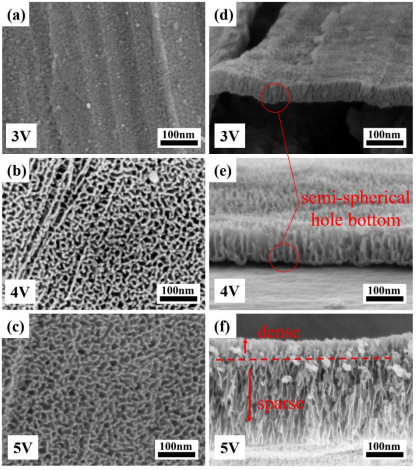
\includegraphics[width=72mm]{img/sample/sem.png}
  \caption{阳极氧化锡在 0.25M NaOH 中，在 3V（a，d），4V（b，e）和 5V（c，f）下阳极氧化 10min 后的 SEM 图像，俯视图（a-c）和横断面图（d-f）}
  \label{fig:sem}
\end{figure}

比电容可按照\njusteqref{eq:specific-capacitance} 计算，其中 $I$ 为放电电流，$\Delta t$ 为放电时间，$m$ 为活性材料质量，$\Delta U$ 为电压窗口。

\begin{equation}
  C_{\mathrm{s}} = \frac{I \Delta t}{m \Delta U}
  \label{eq:specific-capacitance}
\end{equation}

由表~\ref{tab:eis} 可以看出，$R_{\mathrm{L}}$ 随着沉积时间的延长先降低后略有回升，说明界面电荷传输和孔道连续性之间存在折中关系。图~\ref{fig:sem}、图~\ref{fig:workflow} 与表~\ref{tab:eis} 分别演示了位图、矢量图和表格的交叉引用方式。


